\chapter{Educational Synergy in Teaching and Research}\label{appendix:Education}
\section*{Introduction}

This appendix outlines the dual role undertaken during the semester as both a Teaching Assistant (TA) in the course "SW2PLA: Practical Linear Algebra for Software Engineers" and conducting research for a Bachelor's thesis. This unique position facilitated bridging theoretical understanding and practical application, fostering an educational environment where concepts in linear algebra, taught in the SW2PLA course, were directly linked to research in Large Language Models (LLMs).

\section*{Dual Role and Synergistic Learning}

As a Teaching Assistant in the SW2PLA course, responsibilities included assisting students with practical exercises, grading assignments, and engaging in discussions about linear algebra during lectures. These activities aimed to deepen students' understanding of linear algebra's application in modern computational technologies, particularly within the realms of basic AI and elementary machine learning. Simultaneously, the bachelor's thesis focused on integrating linear algebra within the development and optimization of LLMs, specifically assessing the effectiveness of low-rank approximation by SVD of Facebook's BART-model's attention weight matrices. This dual role provided a new perspective on the practical applications of linear algebra in AI research and a further understanding of the linear algebra concepts taught in the SW2PLA course.

\section*{Project Overview in SW2PLA}

The final project for the SW2PLA course required students to undertake a practical application of eigendecomposition or SVD. The project aimed to provide hands-on experience with linear algebra's potent applications, offering several avenues for exploration:

\begin{enumerate}
  \item \textbf{Recommender Systems}: Using SVD to predict user preferences based on past interactions.
  \item \textbf{PageRank Algorithm}: Implementing an eigenvector-based approach to rank web pages.
  \item \textbf{Image Compression}: Applying SVD to reduce the dimensionality of image data without losing significant information.
  \item \textbf{Fibonacci Algorithm}: Using eigendecomposition to compute the Fibonacci algorithm without recursion.
  \item \textbf{Eigenportfolios}: Employing eigendecomposition for optimized stock portfolio selection.
  \item \textbf{Facial Recognition}: Utilizing PCA (a form of eigendecomposition) to identify and classify facial features in images.
  \item \textbf{Open Project}: Any project idea involving Eigendecomposition or SVD, whether applying these techniques to optimize algorithms, enhance data processing, or explore new applications, approaches, or innovative use of linear algebra.
\end{enumerate}

\section*{Integration with Bachelor's Thesis}

During the course, the methodologies and intermediate findings of the bachelor's thesis were presented to the class. This presentation served as a practical demonstration of how linear algebra is utilized within the development and optimization of LLMs—particularly through techniques like low-rank approximations and matrix factorizations—to enhance computational efficiency and model scalability. This further provided students with real-world applications of their theoretical studies.

\section*{Student Projects and Feedback}

The culmination of the course was the student presentations, where they demonstrated their projects' outcomes. This session provided an interactive platform for peer learning and feedback, where students could showcase their application of linear algebra in various projects. The presentation alongside the students' highlighted the reciprocal nature of teaching/learning and research.

\section*{3rd place at the 2024 CLAI Poster Competition}
In addition to sharing findings within the SW2PLA course, the methodologies and intermediate results of the bachelor's thesis were presented at a poster competition held during the 2024 CLAI workshop. This presentation allowed engagement with a broader audience of experts and peers in the field, receiving valuable feedback that furthered research endeavors.

The highlight of this event was the recognition of the work, securing 3rd place in the competition. This achievement not only affirmed the quality and relevance of the research in the field of AI but also provided a platform to showcase the practical applications of linear algebra in optimizing Large Language Models. This external validation brought additional perspective to the educational content delivered in the SW2PLA course, enhancing the overall teaching and learning experience.

\begin{figure}[H]
    \centering
    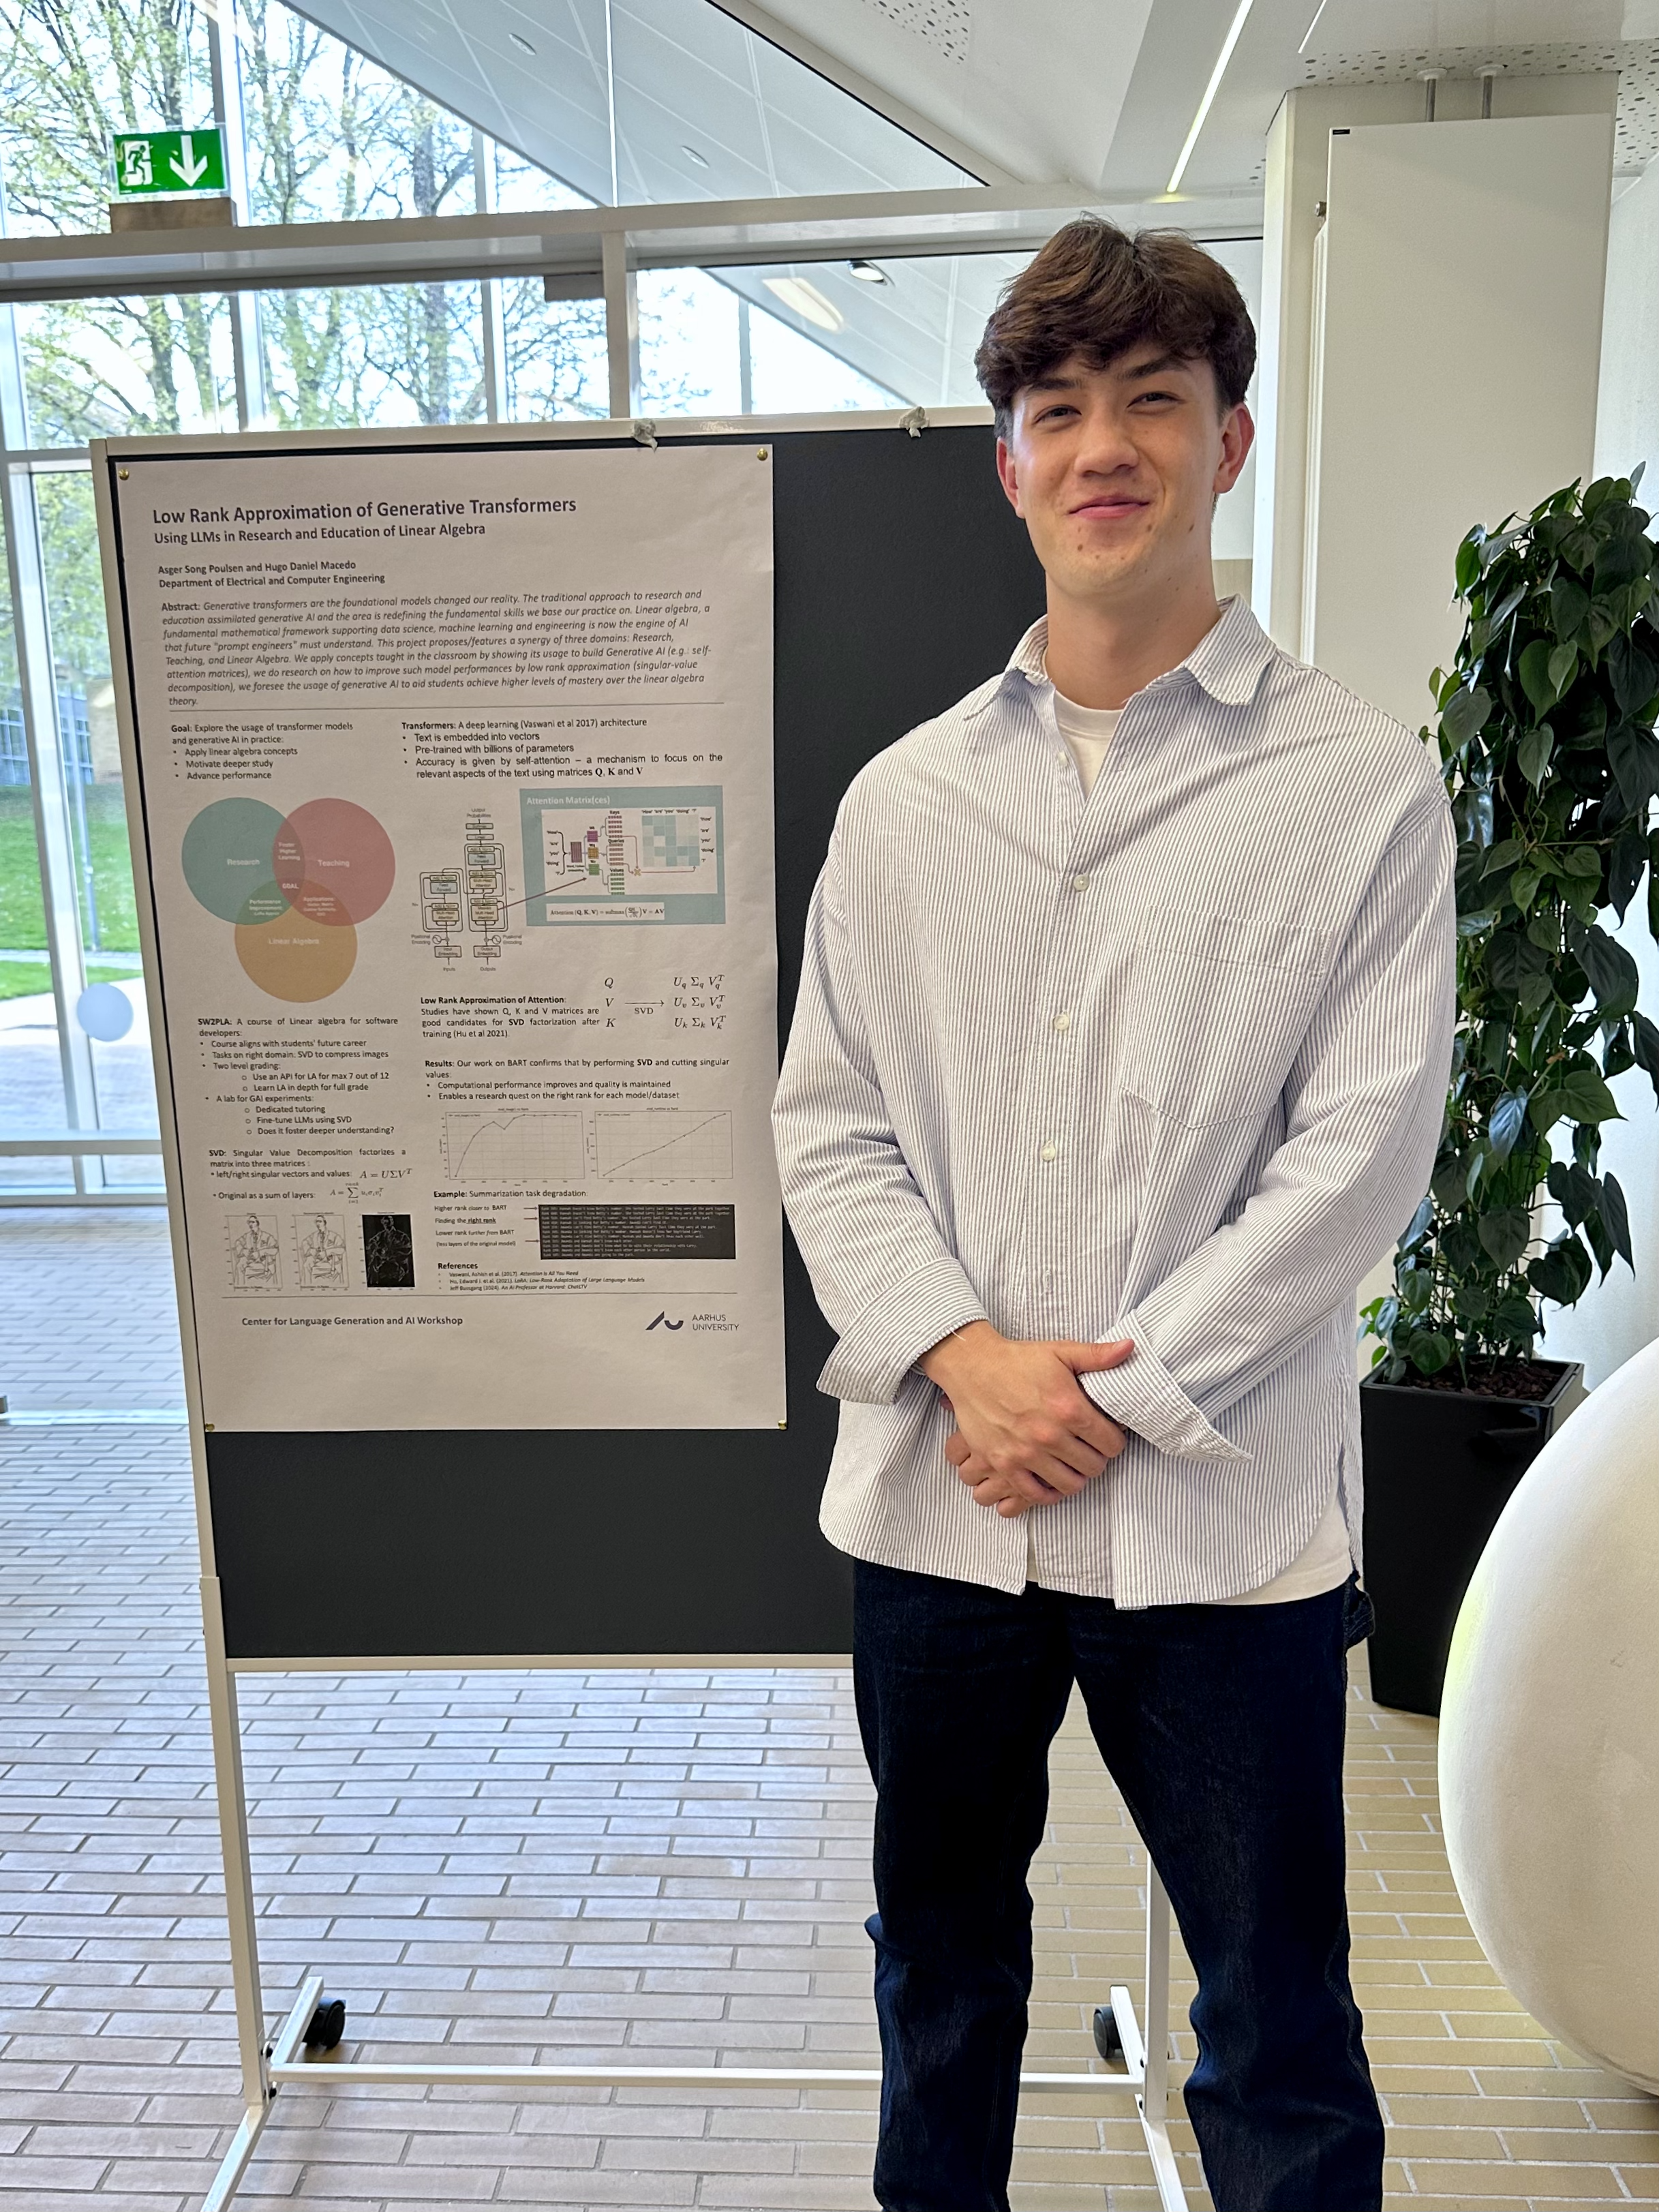
\includegraphics[width=0.6\textwidth]{figs/IMG_5113.png}
    \caption{3rd place in the CLAI Poster Competition}
    \label{fig:CLAI_Poster_Competition}
\end{figure}
It was an honor to represent the Department of Electrical and Computer Engineering (ECE) at such a forum. This accolade not only represents a personal achievement but also served as valuable practice for presenting research findings to a broader audience, including students and faculty members from various disciplines.

\section*{Conclusion}

The involvement in the SW2PLA course as a TA, while simultaneously conducting research for the bachelor's thesis, created a rich educational synergy. This experience not only enhanced the understanding and teaching of linear algebra but also allowed for the direct application and evaluation of theoretical concepts in practical, research-based applications. It underscores the importance of an integrated approach in education, where teaching responsibilities and academic research complement and enrich each other, preparing students for future challenges in technology and engineering.
